% Asset ID: A22StatisticalHypothesisTestingTIKZ-001
% Unit code: A22
% Topic code: A22-HT
% Topic name: Statistical hypothesis testing
% Related lesson section: Key Definitions and Notation, PMCC
% Source: CCEA specification map; lesson transcript; Stats Yr2 Chapter 1 PDF
% Purpose: Show the PMCC scale from -1 to 1 and its linear-correlation interpretation.
% Status: Phase 4 TikZ draft

\documentclass[tikz,border=8pt]{standalone}
\usepackage{amsmath}
\usepackage{tikz}
\usetikzlibrary{arrows.meta, positioning}
\begin{document}
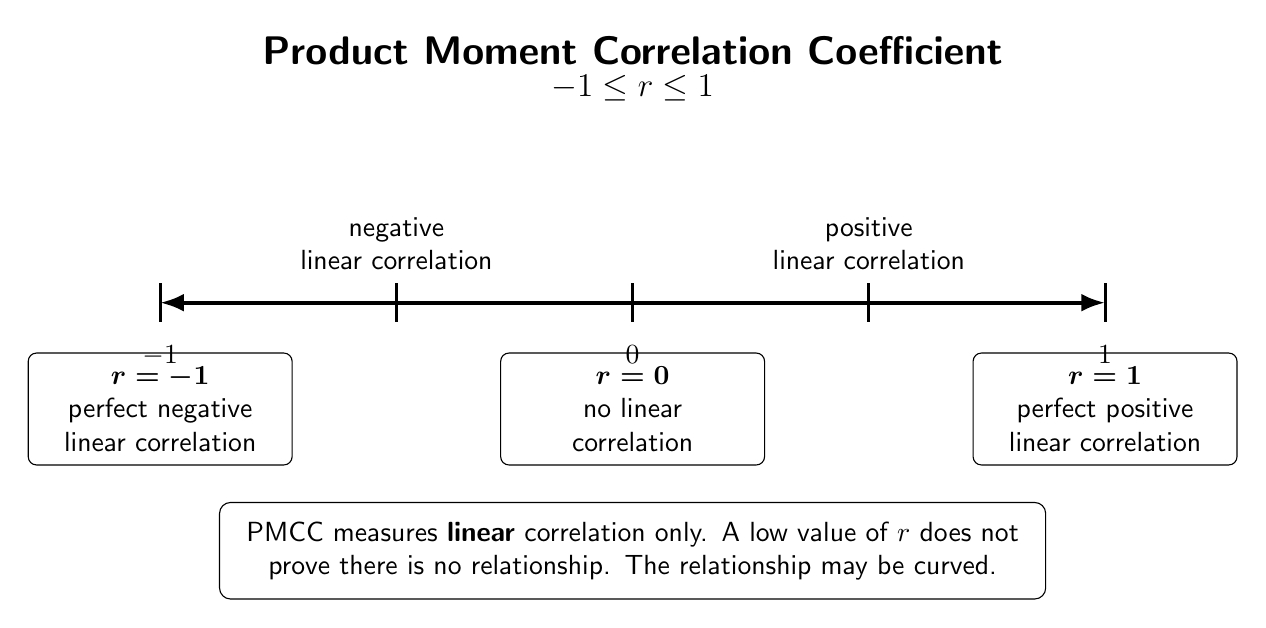
\begin{tikzpicture}[font=\sffamily, axis/.style={line width=1.4pt, -{Latex[length=3mm]}}, tick/.style={line width=1.1pt}, labelbox/.style={draw, rounded corners=3pt, align=center, inner sep=5pt}]
\node[font=\sffamily\bfseries\Large] at (0,3.2){Product Moment Correlation Coefficient};
\node[font=\sffamily\large] at (0,2.72){\(-1 \leq r \leq 1\)};
\draw[line width=1.4pt, {Latex[length=3mm]}-{Latex[length=3mm]}] (-6,0) -- (6,0);
\foreach \x/\lab in {-6/{-1}, -3/{}, 0/{0}, 3/{}, 6/{1}} {\draw[tick] (\x,0.25) -- (\x,-0.25); \node[below=5pt] at (\x,-0.25) {\(\lab\)};}
\node[labelbox, text width=3.0cm] at (-6,-1.35){\(\boldsymbol{r=-1}\)\\perfect negative\\linear correlation};
\node[labelbox, text width=3.0cm] at (0,-1.35){\(\boldsymbol{r=0}\)\\no linear\\correlation};
\node[labelbox, text width=3.0cm] at (6,-1.35){\(\boldsymbol{r=1}\)\\perfect positive\\linear correlation};
\node[align=center] at (-3,0.75){negative\\linear correlation};
\node[align=center] at (3,0.75){positive\\linear correlation};
\node[draw, rounded corners=4pt, text width=10cm, align=center, inner sep=7pt] at (0,-3.15){PMCC measures \textbf{linear} correlation only. A low value of \(r\) does not prove there is no relationship. The relationship may be curved.};
\end{tikzpicture}
\end{document}
